\documentclass[a4paper,12pt]{article}
\usepackage[utf8]{inputenc}
\usepackage{listings}
\usepackage{float}
\usepackage[margin=1in]{geometry}
\setlength\parindent{0pt}
\usepackage{xcolor}
\usepackage{graphicx}
\definecolor{dkgreen}{rgb}{0,0.6,0}
\definecolor{dred}{rgb}{0.545,0,0}
\definecolor{dblue}{rgb}{0,0,0.545}
\definecolor{lgrey}{rgb}{0.9,0.9,0.9}
\definecolor{gray}{rgb}{0.4,0.4,0.4}
\definecolor{darkblue}{rgb}{0.0,0.0,0.6}
\lstdefinelanguage{python}{
      backgroundcolor=\color{lgrey},  
      basicstyle=\footnotesize \ttfamily \color{black} \bfseries,   
      breakatwhitespace=false,       
      breaklines=true,               
      captionpos=b,                   
      commentstyle=\color{dkgreen},   
      deletekeywords={...},          
      escapeinside={\%*}{*)},                  
      frame=single,                  
      language=C++,                
      keywordstyle=\color{purple},  
      morekeywords={BRIEFDescriptorConfig,string,TiXmlNode,DetectorDescriptorConfigContainer,istringstream,cerr,exit}, 
      identifierstyle=\color{black},
      stringstyle=\color{blue},      
      numbers=right,                 
      numbersep=5pt,                  
      numberstyle=\tiny\color{black}, 
      rulecolor=\color{black},        
      showspaces=false,               
      showstringspaces=false,        
      showtabs=false,                
      stepnumber=1,                   
      tabsize=5,                     
      title=\lstname,                 
    }
    
%opening
\title{CS325 Homework 1}
\author{Kabir Kang, Paul Ely, Jason Dorweiler}

\begin{document}

\maketitle

\section{Mathematical Analysis}


\paragraph{Running time analysis of algorithm 1.} The overall asymptotic running time of algorithm 1 is $O(n^3)$. The conditionals at the beginning of the function are constant-time operations. After that it enters into three nested loops. The outer-most loop is $\theta(n)$ since it will always run through the entire set. The inner loops are $O(n)$ each since they will shrink and expand as the algorithm iterates through n. The inner-most loop where the sum of the array slice from e to j is calculated will frequently be much smaller than n. Overall this gives an $O(n^3)$ running time.

  \begin{lstlisting}[language=python,caption={pseudo code for $n^3$ algorithm},mathescape]
if len(array) == 1: # O(1) constant operation
maxSum = array[0] # O(1) constant operation
else:
for e in range(len(array)): # $\theta $(n)
for j in range(e,len(array)): # $\theta$ (n) -- always runs through all elements
maxSum = np.maximum(maxSum, sum(array[e:j])) # O(n) -- shrinks
  \end{lstlisting}

\paragraph{Running time analysis of algorithm 2.} The overall running time for algorithm 2 is $\theta(n^2)$. This algorithm has two nested loops that iterate over n, with the outermost loop running in $\theta(n)$ and the inner loop running in O(n) time. Overall the inner loop will grow smaller as the outer loop counter gets larger, but the running time will tend to be $\theta(n^2)$.
  \begin{lstlisting}[language=python,caption={pseudo code for $n^2$ algorithm},mathescape]
for e in range(len(array)): # $\theta$(n)
testSum = 0 # O(1) constant
for j in range(e,len(array)): # O(n)
testSum += array[j] # O(1) constant
maxSum = np.maximum(maxSum, testSum) # O(1) constant
  \end{lstlisting}

\paragraph{Running time analysis of algorithm 3.} The overall running time for algorithm 3 is $\theta(n log n)$. The $\theta(n)$ running time comes from the portion where it calculates the crossing sum, which involves two $\theta(n)$ operations over the lower and upper halves of n, giving $ \frac{1}{2} \theta(n) + \frac{1}{2} \theta(n)$. The logarithmic portion comes from the recursive calls to calculate the left- and right-sums. These calls divide n in half each time, resulting in $\theta(log n)$ running time. Since the whole function is called recursively, this gives $ \theta(n) * 2 \cdot \theta(log n) = \theta(n log n)$.


  \begin{lstlisting}[language=python,caption={pseudo code for $n\log(n)$ algorithm},mathescape]
def algo3(array):
if(len(array) == 0): # whole block is O(1) operations
return 0
if(len(array) == 1):
return array[0]

mid = len(array)/2 # whole block is O(1) operations
tempL = tempR = 0
maxLeft = maxRight = -infinity

#left side crossing -- mid backwards
for i in range(mid,0,-1): # $\theta(n) / 2$
tempL = tempL + array[i] # constant O(1)
maxLeft = np.maximum(maxLeft, tempL) # constant O(1)

#right side crossing -- mid forwards
for j in range(mid+1, len(array)): # $\theta(n) \div 2 $
tempR = tempR + array[j] # constant O(1)
maxRight = np.maximum(maxRight, tempR) # constant O(1)
maxCrossing = maxLeft + maxRight # constant O(1)

MaxA = algo3(array[:mid]) # $\theta$(n/2) -- halves each time
MaxB = algo3(array[mid+1:]) # $\theta$(n/2) -- halves each time

return np.maximum(np.maximum(MaxA, MaxB),maxCrossing))
  \end{lstlisting}

\section*{Theoretical Correctness}

\section*{Experimental Analysis}

\begin{figure}[h!]
\centering
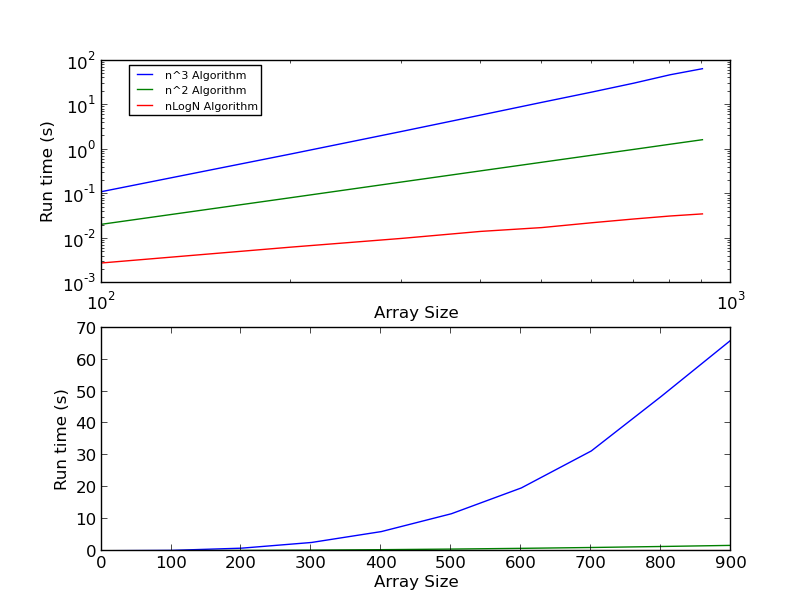
\includegraphics[width=0.8\textwidth]{plotTo900}
\caption{Plot of the three algorithms up to array size of 900, top: log/log, bottom: normal axis}
\end{figure} 

A plot of the run times for the three algorithms are shown in figure 1.  The results of the slope calculation for each algorithm are shown in the table below.  The slope calculation fits with what we would expect.  The $n^3$ algorithm has a slope ~3, the $n^2$ algorithem has a slope ~2, and the $n\log(n)$ algorithm has a slope a bit higher than 1. \\

\begin{tabular}{|c|c|}
\hline 
Algorithm & Slope of log-log plot \\ 
\hline 
$n^3$ & 2.89 \\ 
\hline 
$n^2$ & 1.99 \\ 
\hline 
$n\log(n)$ & 1.16 \\ 
\hline 
\end{tabular}\\

In the lower plot on figure 1 we have also plotted the three algorithms with a normal axis.  This shows the $n^3$ run time of the first algorithm.  The third algorithm runs so quickly that it doesn't even show up at this scale. 

\begin{figure}[h!]
\centering
\includegraphics[width=0.8\textwidth]{plotTo9000}
\caption{Plot of the three algorithms up to array size of 9000, top: log/log, bottom: normal axis}
\end{figure} 



\pagebreak
 

\section*{Extrapolation and Interpretation}

\textbf{What is the biggest instance that you could solve with your algorithm in one hour}\\

From our experimental data and using the slope of our log-log plot we determined that the relationship between run time and array size for the $n\log(n)$ algorithm is approximately: 
$$\log(time) = 1.16\log(elements)- 11.15$$

Using this equation and a run time of 1 hr (3600s) we get an approximate array size of 17.4 million elements \\


\textbf{Determine the slope of the line in your log-log plot and from these slopes infer the experimental running time for each algorithm. Discuss any discrepancies between the experimental and theoretical running times}\\

\end{document} 
